\documentclass[9pt,twocolumn,twoside]{osajnl}
%% Please use 11pt if submitting to AOP
% \documentclass[11pt,twocolumn,twoside]{osajnl}

\journal{ol} % Choose journal (ao,jocn,josaa,josab,ol,optica,pr)

%See template introduction for guidance on setting shortarticle option
\setboolean{shortarticle}{true}
% true = letter/tutorial
% false = research/review article
% (depending on journal)


\usepackage{lineno}
\usepackage{siunitx}
\usepackage{float}
\usepackage{lipsum}

\newcommand{\inred}[1]{{\color{red}#1}}

\linenumbers


\title{Beam focus modifications by cropping partially coherent X-ray beams}


\author[1*]{Manuel Sanchez del Rio}
\author[1]{Rafael Celestre}
\author[1]{Juan Reyes-Herrera}
\author[1]{Philipp Brumund}
\author[1]{Marco Cammarata}

\affil[1]{European Synchrotron Radiation Facility, 71 Avenue des Martyrs, 38000 Grenoble}

\affil[*]{Corresponding author: srio@esrf.eu}

\begin{abstract}
We simulate the focusing of a partially-coherent X-ray beam emitted by an undulator in a fourth-generation storage ring performing coherent mode decomposition and wave optics propagation. The focus position is shifted, and its size is enlarged when an entrance slit crops the beam. 
This is the usual case when a slit crops the beam (notably to select the coherent fraction).
% One important role of the aperture is to select the coherent fraction of the beam. 
The pairing of two focusing elements (mirrors, lenses or transfocators) to ensure a fixed focal position is also analyzed. Our results show that the image of a partially coherent source, such an undulator in a low-emittance storage ring, is a non-trivial function of the aperture used to control the coherence fraction.
\end{abstract}

\setboolean{displaycopyright}{true}

\begin{document}

\maketitle

\section{Introduction}
\label{sec:introduction}
Fourth-generation storage-ring-based X-ray synchrotron sources deliver photon beams with high brilliance and coherence. Although the transverse coherence of these beams is highly improved in the horizontal direction, 
the overall coherent fraction is of the order of a few per cent for hard X-rays ($>10$~keV). Beamline optical elements such as pinholes and slits are then used to improve coherent fraction to values typically $>80 \%$ needed for applications exploiting coherence, such as X-ray photon correlation spectroscopy, coherent diffraction imaging, propagation-based phase-contrast imaging, and ptychography \cite{paganin_book}. The coherent beam interaction with the optical elements produce diffraction, thus modifying the beam characteristics and also affecting the beam focusing, as discussed here.

Let us consider the case of an ideally focusing system of focal length $f$ (made by a mirror or lens that focuses the source into the image plane). The position of the focus with respect to the focusing element $q$ is given, in the framework of geometric optics, by the lens equation $f^{-1}=p^{-1}+q^{-1}$, with $p$ the source-element distance. If the numerical aperture (NA) of the beam is reduced (for example by the finite dimension of the lens or mirror, or by using a slit) the location and dimension of the focus change as a result of diffraction. It has been shown \cite{Tanaka:85} that the focal position of a Gaussian beam ``moves" towards the lens position when the NA decreases. This shifting of the focal position is relevant for synchrotron beamlines, as demonstrated by Westfahl {\it et al.} \cite{westfahl}. These authors noticed a shift of the horizontal focal position upstream from the position given by geometrical optics (Fig. 7 ibid.) when the horizontal acceptance is reduced by a slit. 

The diffraction effect at the slits and finite size of the optical elements not only shifts the focal position (up- or downstream), but also changes the focal dimensions. These facts must be taken into account in beamlines in fourth-generation synchrotron sources. They are critical when designing beamlines with several coupled focusing elements. We studied this phenomenon in the context of the project for the new ``EBSL1'' beamline at the upgraded EBS-ESRF storage ring. This beamline will produce highly coherent beams of variable cross section at the sample position. Two refractive systems (transfocators) will be paired to allow a varying focal size, whereas a slit placed upstream from the transfocators is used to control the coherent fraction. The optical matching of the transfocators is strongly correlated to the slit aperture (or coherent fraction). The performances of such systems are calculated in the framework of the partially coherent optics using a fast algorithm for decomposition of the undulator radiation in coherent modes that are propagated along the beamline using the algorithms presented in \cite{delrio2021pairing}. The idoneity of this method is discussed (ibid.) and compared with other partial coherence simulation algorithms. The key point is to treat separately the horizontal and vertical planes, therefore working with one-dimensional wavefronts.

\section{Focal position produced by a single focusing element}
\label{sec:onelens}

%%%%%%%%%%%%%%%%%%%%%%%%%%%%%%%%%%%%%%%%%%%%%
% \onecolumn
\begin{figure*}[t]
\hspace*{-1.0cm}
\centering
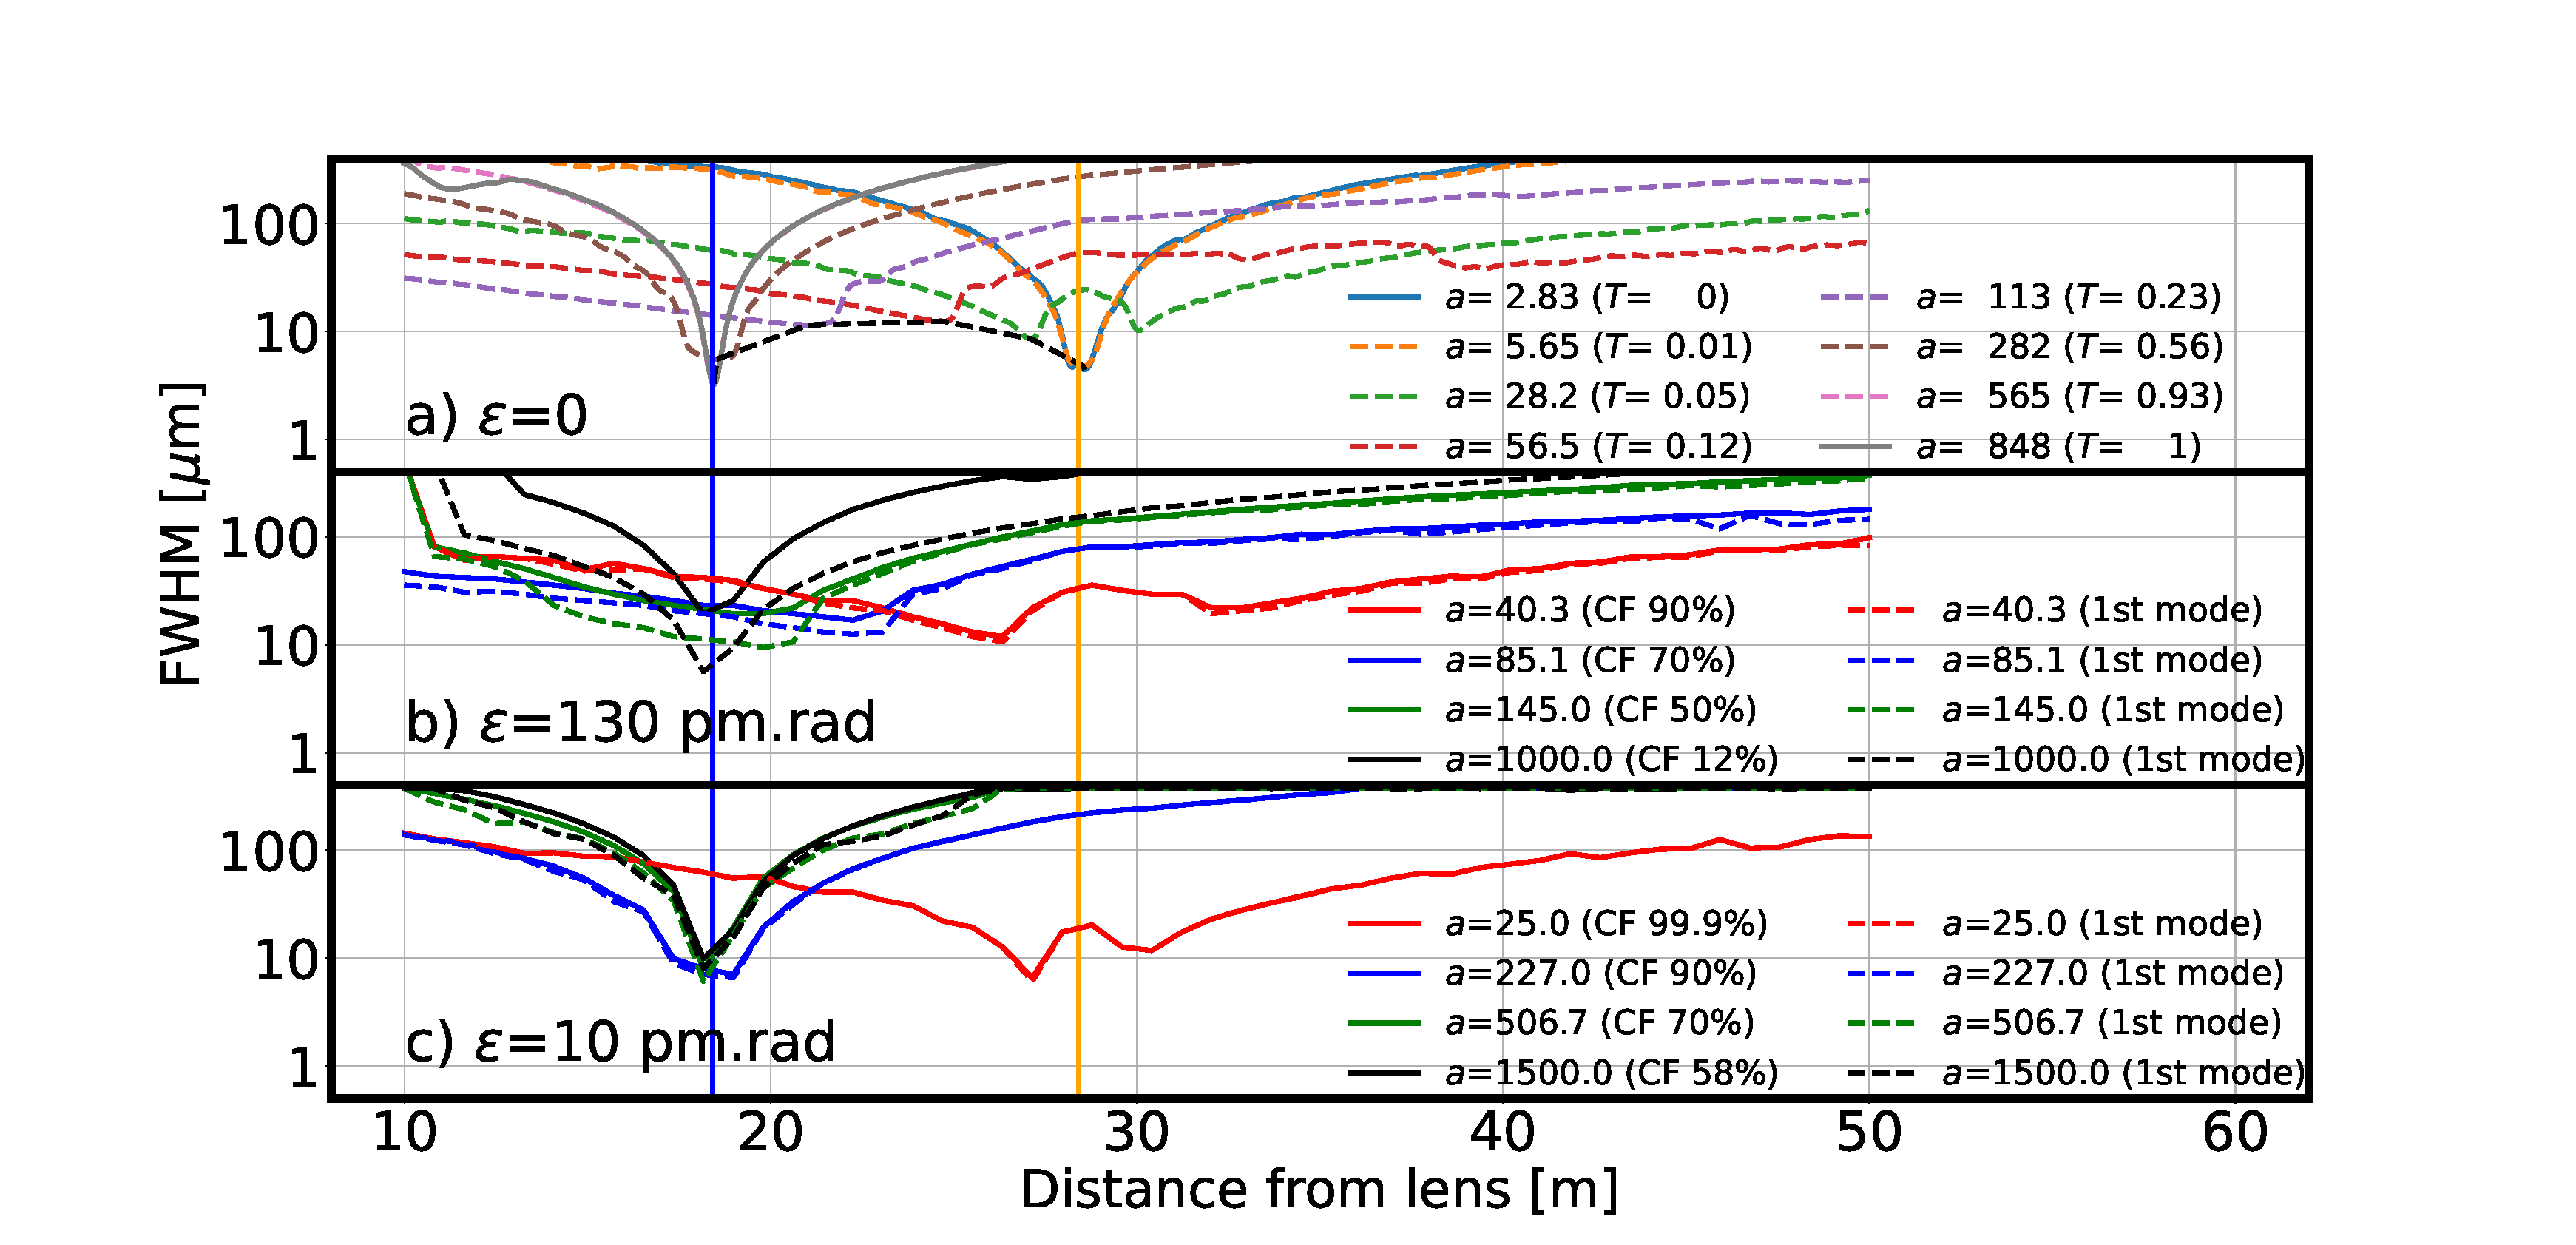
\includegraphics[width=0.8\textwidth]{figures/evolution.eps}
\caption{Evolution of the size of an undulator beam cropped by a slit and focused by a lens of $R=\SI{0.2}{\milli\meter}$.
The plots show the FWHM of the beam as a function of the distance from the lens for different values of the aperture $a$ (in \SI{}{\micro\meter}). 
a) Zero emittance case ($\varepsilon=0$, full coherence),
b) horizontal emittance ($\varepsilon=130$~pm.rad) and c) vertical emittance ($\varepsilon=10$~pm.rad) for the EBS-ESRF storage ring.
The focal positions given by geometrical optics when the source is considered at either the undulator position (blue vertical line at $q$) or at the slit position (orange vertical line at $q_a$) are marked.
Full lines in b), c) correspond to partial coherent (multi-mode) beam, whereas the dashed lines correspond to the full coherent beam (first mode).
}
\label{fig:oneTFund}
\end{figure*}
% \twocolumn
%%%%%%%%%%%%%%%%%%%%%%%%%%%%%%%%%%%%%%%%%%%%%

Let us consider an aperture of dimension $a$ placed between the source and a focusing optical element (here we consider a lens), at a distance $p_a$ from the lens ($p_a < p$). The lens is set to focus the source into an image plane at $q$ downstream from the lens. Following the geometrical optics, the position of the focal plane is defined by the lens equation (which does not depend the aperture $a$), and the focal size is $M \times s$  (considering the aperture size $a$ is larger than the source size $s$). $M = q/p$ is the optical magnification. If $a$ is smaller than the beam size, the aperture obscures part of the source reducing the beam intensity. However, the focal size and focal position (where the beam waist is found) are not modified. When the beam has a high coherence, these results predicted by geometrical optics are insufficient \cite{hierarchical}. This section presents a numerical study of the position and size of the beam waist for different apertures taking into account the partial coherence of undulator emission. We simulated a U18 undulator (period $\lambda_u=\SI{18}{\milli\meter}$) with $N_u=138$ periods. The gap is tuned to have the first harmonic at $E=7$~keV (deflecting parameter $K=1.851$). We consider a Be lens with parabolic profile and radius at the appex $R=\SI{0.2}{\milli\meter}$ ($f=\SI{14.35}{\meter}$ at 7~keV), located at a distance $p=\SI{65}{\meter}$ from the source. A slit of variable aperture $a$ is placed at $p_a=\SI{29}{\meter}$ upstream from the lens. 

We first suppose an ideal storage ring with zero emittance, therefore producing a fully coherent emission. The beam at the slit plane has a full-width at half-maximum (FWHM) $a_\text{FWHM}=~\SI{565}{\micro\meter}$. The aperture $a$ takes different values from fully opening (the whole beam passes the slit therefore the transmittivity is $T=1$) to a very narrow aperture ($T\ll1$). The refracted beam is analyzed at different positions from the lens by calculating the FWHM of the intensity distribution. At the beam waist the FWHM presents a minimum. 

Fig.~\ref{fig:oneTFund}a shows the evolution of the coherent beam size after being focused by the lens. It also shows markers for the focal positions predicted by the lens equation:  $q=\SI{18.417}{\meter}$ considering the source at the undulator position (blue line) and $q_a=\SI{28.408}{\meter}$ if one considers the slit as an effective source (orange line). As expected, the beam waist calculated numerically converges to these respective values when the slit is opened ($T=1$, Fresnel number $N_F=78$, grey line) and almost closed ($T\approx0$, blue line). For intermediate values of $a$, the beam waist ``moves" from one case to another. For $T=0.93$ ($N_F=35$, magenta line) the cropping by the slit is negligible so situation does not change with respect the open slit. For $T=0.56$ ($N_F=8.7$, brown line) the waist presents a flat depression, increasing its minimum FWHM and also the depth of focus. Smaller values of $T$ and $N_F$ shift the minimum to higher distances (e.g., $T=0.12$, $N_F=0.3$,  red line) and the minima become less pronounced. A small FWHM is found close to $q_a$ (orange marker) for $T=0.05$ ($N_F=0.09$, green line), showing a twin minimum due to the interference fringes found in the intensity distributions. Both minima converge to this position for $T=0.01$ ($N_F=0.003$, orange line), and $T=0.003\approx0$ ($N_F=0.0009$, blue line). 
The numeric values of the FWHM agree with those calculated using geometrical concepts only for the limiting cases of waist at $q$ and $q_a$. 
However, for intermediate slit apertures, where the waist position is in between $q$ and $q_a$, the waist size is different to that predicted by geometric optics, and significantly higher that the limiting values at $q$ and $q_a$, showing the envelope in Fig.~\ref{fig:oneTFund}a (dashed black line).
This is an important fact: a good focusing, i.e., a very small beam size is only obtained in the limiting cases of open slit and almost-closed slit. This means that for a fully coherent beam, the slit worsens the focusing. The diffraction at the slit creates a spurious divergence that affects the lens focusing. 
When the focal distance of the lens is reduced (using lenses with smaller radius, or piling several lenses), the $q$ and $q_a$ positions shift to shorter distances, and become closer one to another ($|q-q_a|$ also reduces). They converge to a single position: the lens focal length $q=q_a=f$. This happens when both source-lens and slit-lens distances can be considered at infinite. 

We used the EBS-ESRF emittance values\footnote{Throughout this work we used the electron beam sizes and divergences at the center of the straight section: $\sigma_x=\SI{29.7}{\micro\meter}$,
$\sigma_{x'}=\SI{4.37}{\micro\radian}$,
$\sigma_y=\SI{5.29}{\micro\meter}$,
$\sigma_{y'}=\SI{1.89}{\micro\radian}$, corresponding to beam emittances:  $\varepsilon_x=\SI{130}{\pico\meter \radian}$,
$\varepsilon_y=\SI{10}{\pico\meter \radian}$, and beta functions
$\beta_x=\SI{6.8}{\meter}$,
$\beta_y=\SI{2.8}{\meter}$.
}
to perform the coherent mode decomposition of the undulator source. The details for that are presented in \cite{delrio2021pairing}.
This is done for the horizontal and vertical directions, resulting coherent fractions (at 7 keV) $CF_h=13\%$ and $CF_v=58\%$, respectively. These values are much higher than for the old ESRF-1 source, but still low to apply full-coherence approximation. Therefore, we propagated a number of modes large enough to contain more than 99\% of the source intensity (36 modes in H and 8 in V). The illumination at the entrance slit plane is \SI{610}{\micro\meter} (H) $\times$ \SI{566}{\micro\meter} (V). The slit aperture is effectively used to tune the coherence of the beam: closing the slit increases the $CF$. In the limit (zero aperture) the beam after the slit is fully coherent ($CF=1$), but obviously with zero transmittivity ($T=0$). The choice of the right slit aperture comes from a compromise between coherence and flux.
Figures~\ref{fig:oneTFund}b and~\ref{fig:oneTFund}c show the focal size along the optical axis for several apertures in the horizontal and vertical planes. We calculated the case of the partially coherent beam (multi-mode, solid lines) and also the case of a fully coherent beam (only the first coherent mode, dashed lines). We observe that the focal positions (the minima of the plot lines) do not change significantly when passing from full to partial coherence. However, the focal dimension changes significantly in the horizontal direction for cases with $CF_h\le~70\%$. In the vertical, where the beam at the source was more coherent, there is no much difference in sizes when going from full (dashed lines) to partial coherence (solid lines). Looking to the focal position shift versus $q_a$ (orange marker) we find important differences in the horizontal and vertical.
% \inred{The cropping of the beam by the slit is important in horizontal as we need to increase the $CF_h$ from the source (13\%) to values required by the experiments, usually larger than 50\%.}
Closing the slit produces a gradual shift of the focal position from the position of the geometrical image of the undulator source (blue vertical line) to the geometrical image of the slit (orange vertical line). However, in the vertical plane, the slit crops the beam only slightly, and closing the slit to go from the source $CF_v=58\%$ to values up to 90\% does not produce any focal shift from the position of the geometrical image of the undulator source. Only when the slit is very closed (e.g., $a_v=\SI{25}{\micro\meter}$, red curve) the focal position shifts to the geometrical image of the slit. This case is in principle not interesting experimentally as it reduces the intensity from an already quite coherent beam ($CF_v=90\%$).
In summary, for practical values of aperture selected to increase the beam $CF$ to values ~90\% the behaviour in vertical (V) and horizontal (H) directions is different: the better source coherence in V permits working with quite open slits thus the focusing system "sees" the source at the undulator position, whereas in H one needs a significant crop of the beam thus shifting and enlarging the beam waist. Notice that the good coherence of the beams emitted by the EBS-ESRF and other 4$^{\text{th}}$ generation storage permits performing coherence experiments with a "conservative" use of slit (open in V and partially close in H). On the contrary, these experiments at 3$^{\text{rd}}$ generation sources require a drastic closing of the slits to a pinhole size.      

%%%%%%%%%%%%%%%%%%%%%%%%%%%%%%%%%%%%%%%%%%%%%
\begin{figure}[htbp]
~~~~a)~~~~~~~~~~~~~~~~~~~~~~~~~~~~~~~~~~~~~~~~~~~~~~~~~~~~~~b) \\
\hspace{-1.1cm}
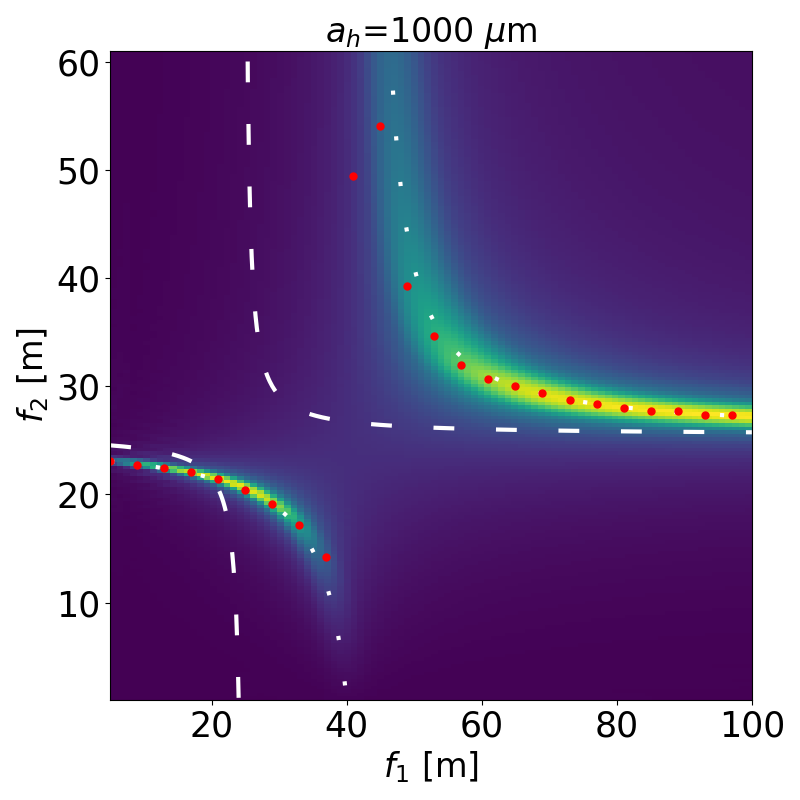
\includegraphics[width=0.25\textwidth]{figures/H_3.png}
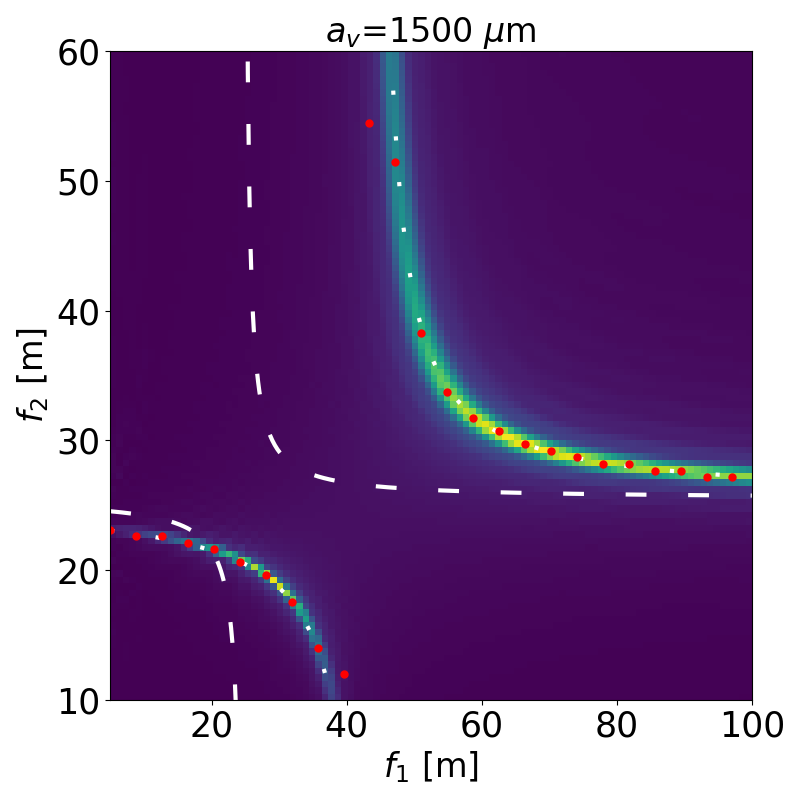
\includegraphics[width=0.25\textwidth]{figures/V_3.png}
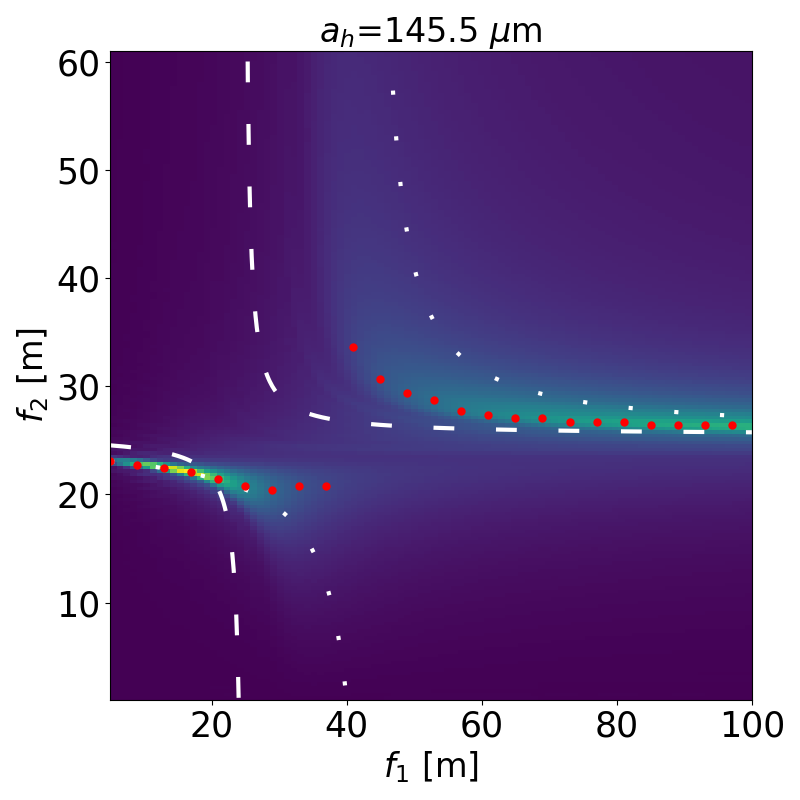
\includegraphics[width=0.25\textwidth]{figures/H_2.png}
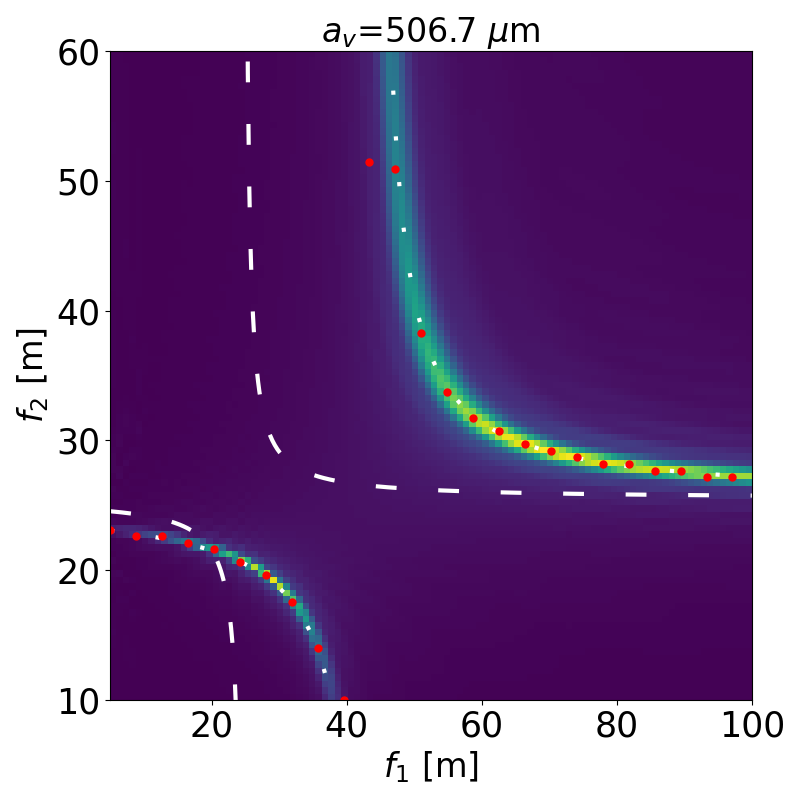
\includegraphics[width=0.25\textwidth]{figures/V_2.png}
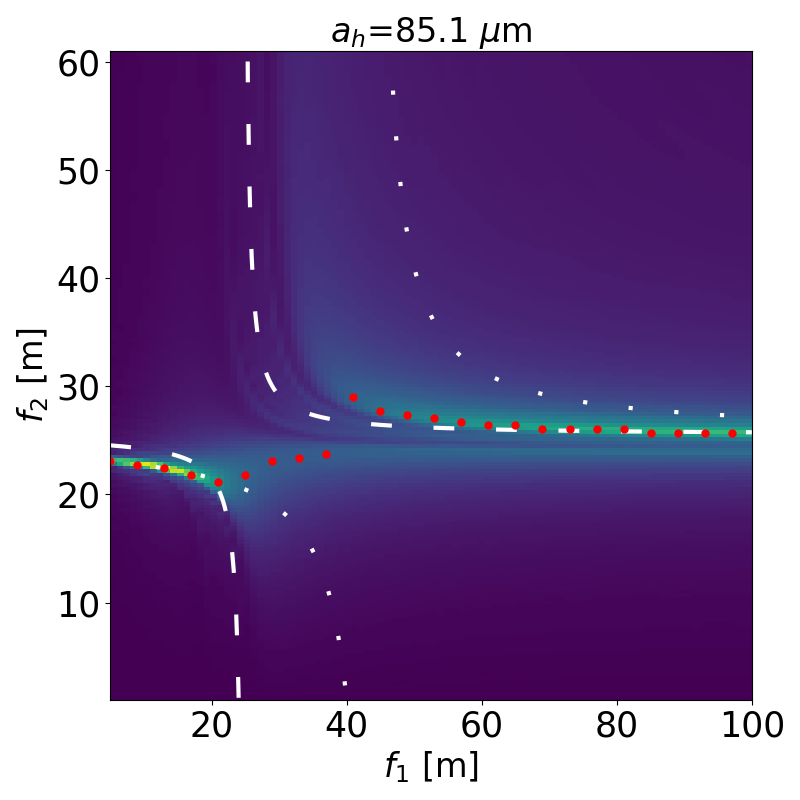
\includegraphics[width=0.25\textwidth]{figures/H_1.png}
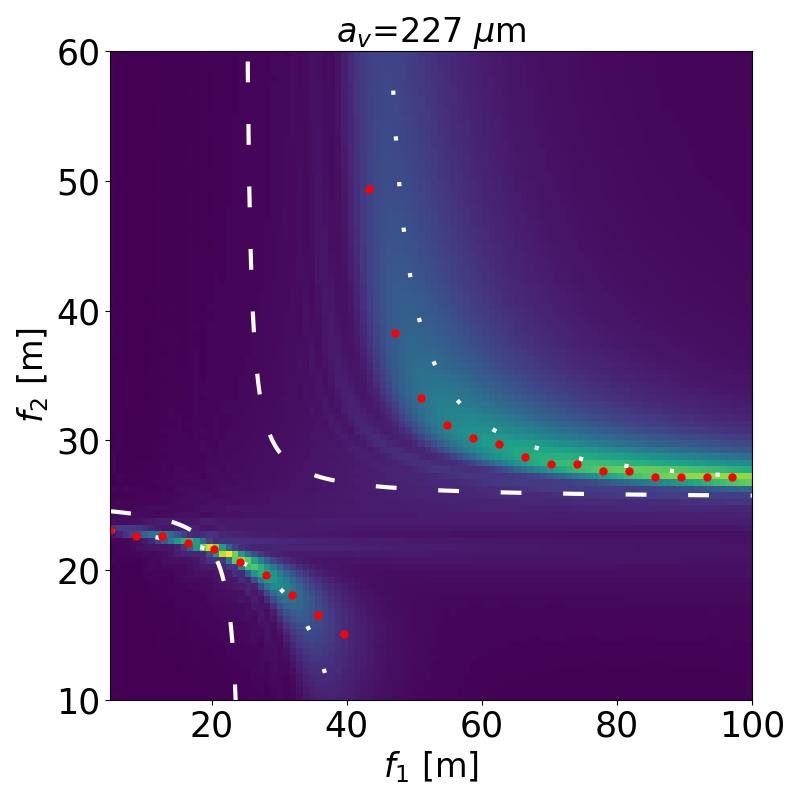
\includegraphics[width=0.25\textwidth]{figures/V_1.png}
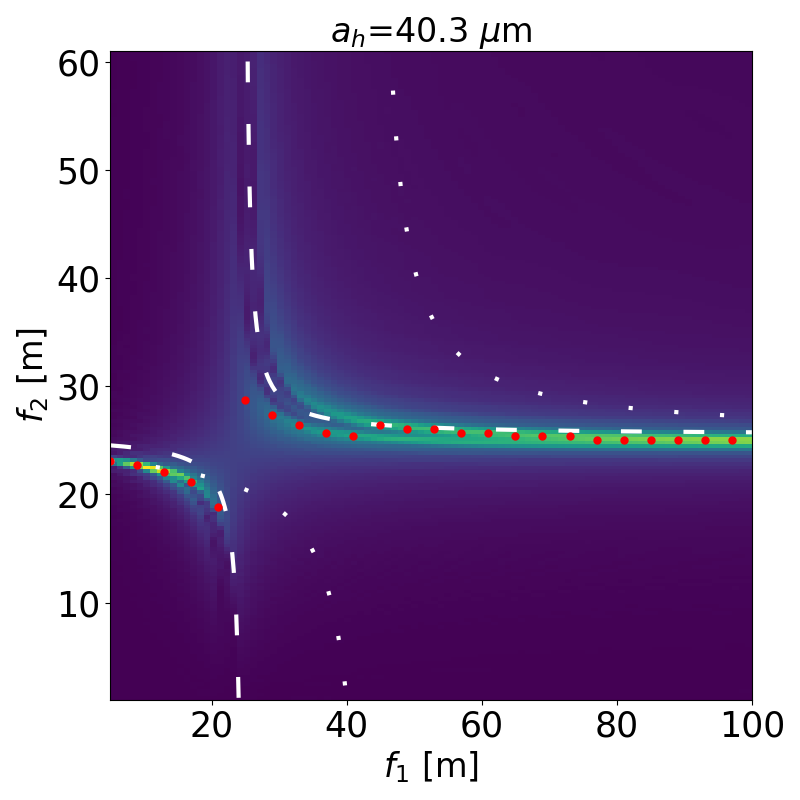
\includegraphics[width=0.25\textwidth]{figures/H_0.png}
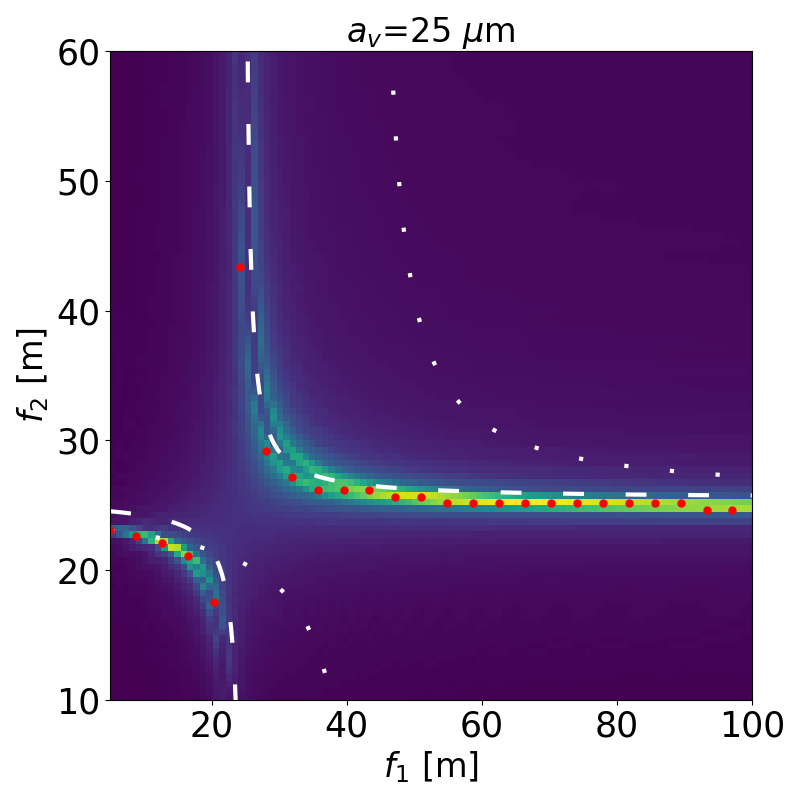
\includegraphics[width=0.25\textwidth]{figures/V_0.png}
\caption{
        \label{fig:f1f2map}
    Maps of beam peak intensity in horizontal plane (column a) and vertical plane (b) at the sample position obtained by two lenses of variable focal lengths ($f_1$,$f_2$).
    Slit values (in \SI{}{\micro\meter}) are $a_h=[1000, 145.5, 85.1, 40.3]$ (a) and $a_v=[1500, 506.7, 227.0, 25]$ (b), corresponding to transmitted coherence fraction
    $CF_h=[0.13, 0.5, 0.7, 0.9]$ and
    $CF_v=[0.58, 0.7, 0.9, 0.999]$, respectively.
    The analytical trajectories from geometric optics (Eq.~\ref{eq:twolens}) are over-plotted in white (dotted if source is at the undulator, and dashed if source is at the slit). We represented in red dots some optimum pairs ($f_1,f_2$) that guarantees that the beam waist is at the focal plane.
    }
\end{figure}
%%%%%%%%%%%%%%%%%%%%%%%%%%%%%%%%%%%%%%%%%%%%%

\section{Focal lengths and sizes for paired focusing elements}

Consider an ideal optical system composed by two focusing elements defined by focal lengths $f_1$ and $f_2$, separated by a distance $D$. Following \cite{Goodman85}, the relationship between object-to-element-1 distance $p_1$ and the element-2-to-image distance $q_2$ given by the geometrical optics is:
\begin{equation}
\label{eq:twolens}
    D-(f_1+f_2)=\frac{f_1^2}{p_1-f_1} + \frac{f_2^2}{q_2-f_2},
\end{equation}
which corresponds to an hyperbola
\footnote{Expanding eq.~\ref{eq:twolens} one gets $x(D q_2 + p_1 q_2) + y (D p_1 + p_1 q_2) - x y (D + p1 + q_2) = D p_1 q_2$,  with horizontal asymptote at $f_{2}=((p_1+D)^{-1}+q_2^{-1})^{-1}$ and vertical asymptote at $f_{1}=(p_1^{-1}+D^{-1})^{-1}$.} in the ($f_1,f_2$) plane.
The global magnification is the product of the magnification of the individual focusing elements.
\begin{equation}
\label{eq:magnification}
    M=M_1 M_2=\frac{1-q_2/f_2}{1-p_1/f_1}.
\end{equation}
The magnification is not dependent on $D$, however the optical throw (length of the optical system $L=p_1+D+q_2$) will change if one changes the focal distances of the elements. For a constant $L$ one can change magnification by changing the inter-element distance $D$ (zoom effect). In a synchrotron beamline, the transfocators are refractive focusing elements that allow changing the magnification by varying their focal lengths (by adding or removing lenses) \cite{Vaughan:kv5084}. Alternatively, two Kirkpatrick-Baez systems with bendable mirrors or multilayers can be used. 



We consider an optical system made by two paired transfocators to get a variable magnification (variable focal size) in a fixed location (the sample position). The configuration match the requirements of the EBS-ESRF EBSL1 beamline. 
The source is a U18 undulator tuned at photon energy of \SI{7}{keV} (as used before). A slit of aperture $a_h \times a_v$ is placed at \SI{36}{\meter} from the undulator.  
We represent the two transfocators by two real beryllium lenses of variable curvature radius $R_1$ and $R_2$ that correspond to focal distances $f_1$ and $f_2$, with $f_{1,2}=R_{1,2}/(2 \delta)$, $\delta=6.96\times10^{-6}$ for Be at \SI{7}{keV}. Lens-1 is placed at $p_1=\SI{65}{\meter}$ from the source, and lens-2 at $D=\SI{105}{\meter}$ downstream from lens-1. The image plane, where sample is placed, is at $q_2=\SI{30}{\meter}$ downstream from the lens-2. The optical throw is $L=p_1+D+q_2=\SI{200}{\meter}$. The slit is $p_a=\SI{29}{\meter}$ upstream from lens-1 (i.e. at \SI{36}{\meter} from the undulator). 
% The positions of the lenses, determined by room constraints, are fixed (although different values could be studied). 

For a given value of $f_1$ and the the fixed distances ($p_1$, $D$ and $q_2$), $f_2$ can be calculated analytically with equation~(\ref{eq:twolens}). The trajectory pairs ($f_1,f_2$) obtained in this way guarantees that the focus is at the sample position ($L=\SI{200}{\meter}$ from source). However, as shown in the previous section, these results of the geometrical optics are not exact when partially coherent beams are cropped by a slit. 
Figure~\ref{fig:f1f2map} shows the results of the numerical search of the $f_2$ to produce the waist at the sample plane. It is obtained by performing a map of the on-axis intensity $\mathcal{I}_0$ of the beam at the sample plane versus $(f_1,f_2)$. Each pixel corresponds to a simulation to compute the pattern at the image plane, considering partial coherence, i.e., propagating many coherent modes. For a given $f_1$ value, one can select the $f_2$ value that produces the best focus at the sample position (picking the maximum of $\mathcal{I}_0(f_2)$, which also corresponds to the minimum FWHM). 
The $\mathcal{I}_0(f_1,f_2)$ maps depend strongly on the slit aperture. In the horizontal, the low $CF_h$ of the source (13\%) is strongly increased when the the slit is being closed, producing appreciable displacement of the pattern in Fig.~\ref{fig:f1f2map}a, thus requiring a fine tuning of $f_2$ to keep the beam focused at the sample plane. In vertical, the source is more coherent ($CF_v=58\%$) and closing the slit does not 
% therefore when the slit improves crops the beam and  enhances the $CF_v$ there is not much 
shift the waist position until reaching $CF_v\approx90\%$. However, when the slit almost closed ($a_v=\SI{25}{\micro\meter}$), that is, acting as a pinhole the patterns approach the ($f_1,f_2$) trajectories resulting from the geometrical optics considering the source at the slit position.

Figure~\ref{fig:focalSizes} shows the calculated focal sizes. Analytical values (dashed lines), based on geometrical optics, i.e. equation~(\ref{eq:magnification}), are close to numeric values of beam sizes for the limiting cases of open slit (source at the undulator) or almost-closed slit (source at the slit). For other useful cases where the slit crops partially the beam, the numerically calculated values should be used. Here, the focal sizes cannot be predicted by geometrical optics (also seen in Fig.~\ref{fig:oneTFund}a), and cannot be simply interpolated from the sizes corresponding to the limiting slit openings. The size values calculated analytically have very limited applicability for practical cases were the beam is partially cropped by the slit. 

%%%%%%%%%%%%%%%%%%%%%%%%%%%%%%%%%%%%%%%%%%%%%%%%%%%%%%%%%%%%%%%%%%%%%%
\begin{figure}[H]
a)\\
\hspace{-2.0cm}
    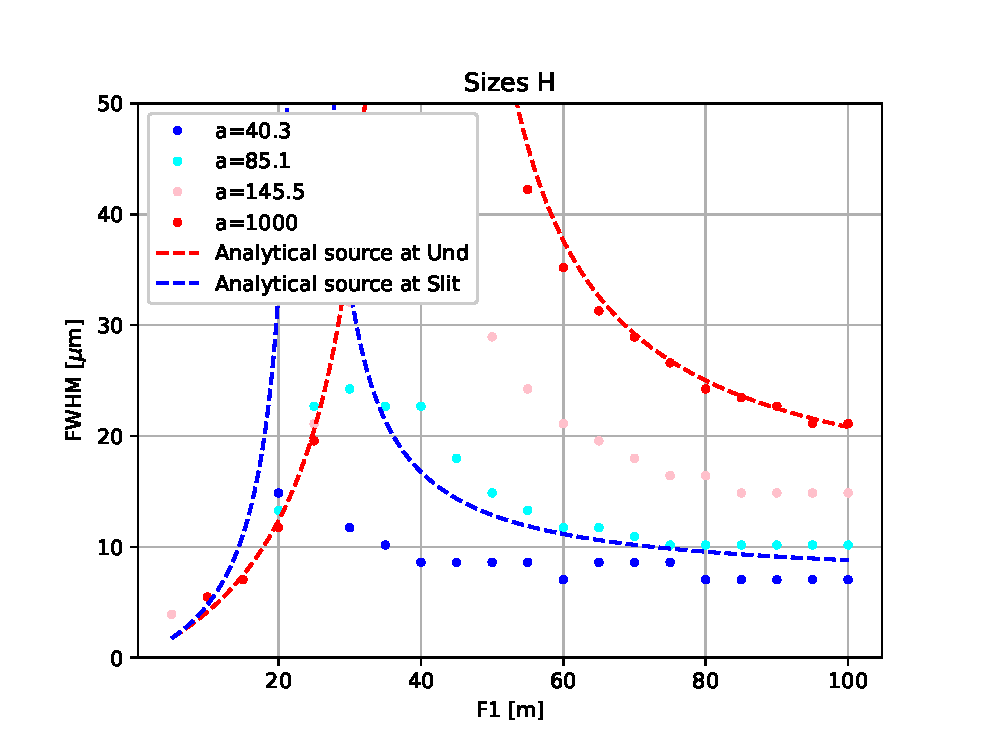
\includegraphics[width=0.40\textwidth]{figures/sizes_h.eps}\\
b)\\
\hspace{-2.0cm}
    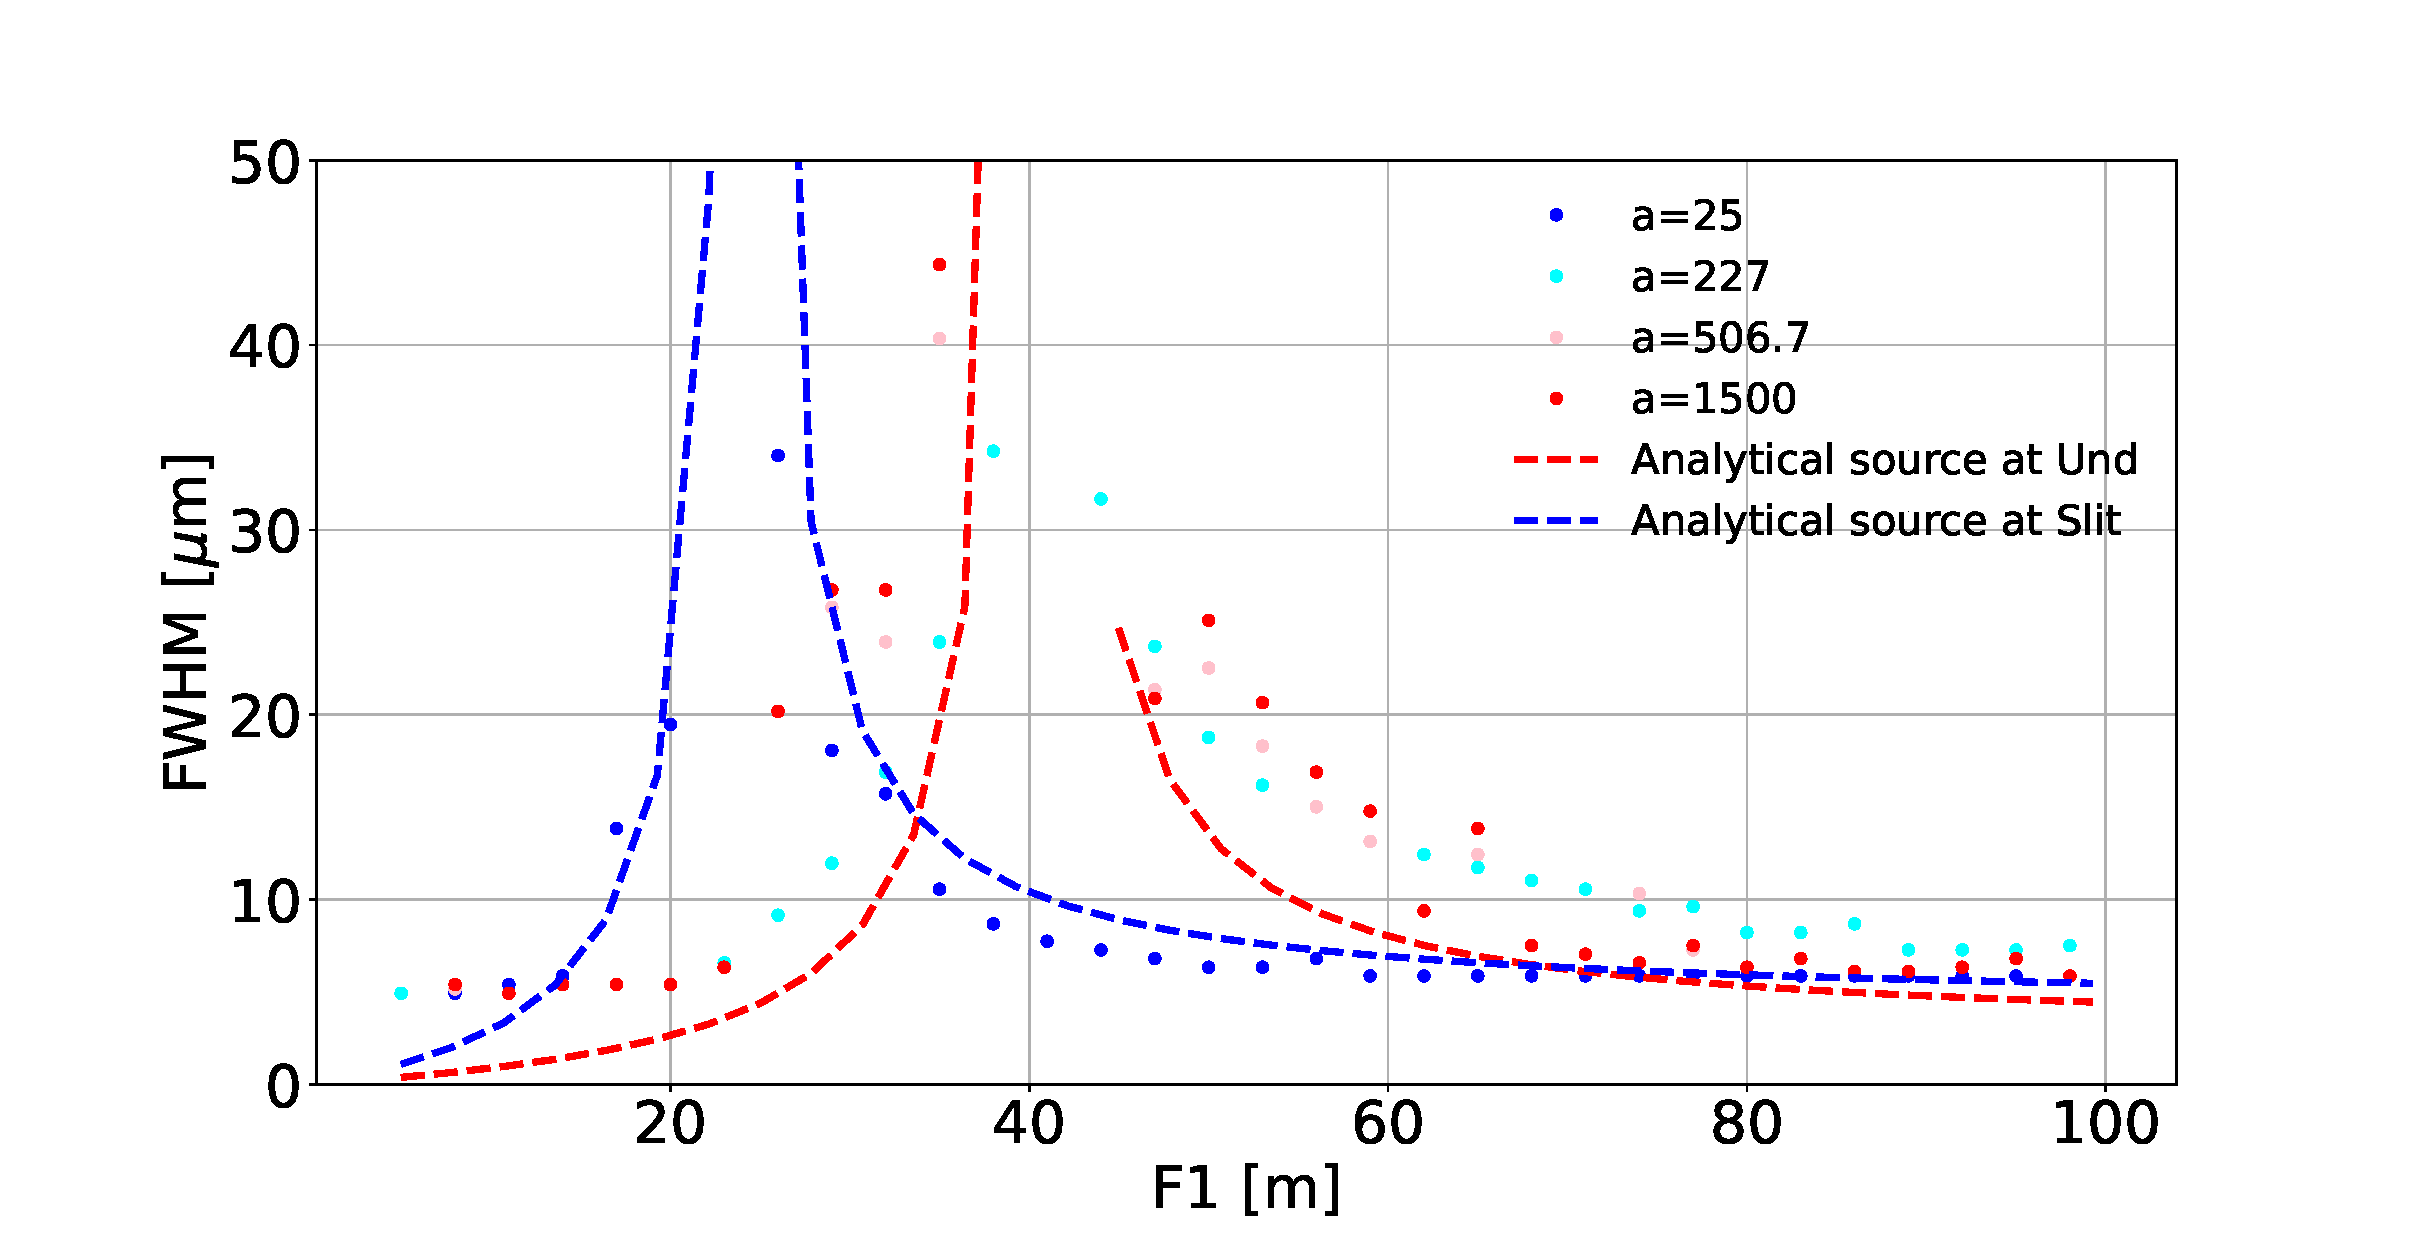
\includegraphics[width=0.40\textwidth]{figures/sizes_v.eps}

    \caption{
    \label{fig:focalSizes}
    Size of the image in a) horizontal and b) vertical planes for different slit apertures.
    }
\end{figure}
%%%%%%%%%%%%%%%%%%%%%%%%%%%%%%%%%%%%%%%%%%%%%%%%%%%%%%%%%%%%%%%%%%%%%%

In the horizontal direction, for slit apertures $a_h>\SI{40}{\micro\meter}$ the sizes change considerably for small changes in $a_h$. The focusing characteristics of the system highly depends on the diffraction effects produced at the slit. For the slit $a_h=\SI{40.3}{\micro\meter}$ ($CF_h=90\%$) the focal size can vary from roughly 10 to 50 microns. In vertical the focal size can be changed from 5 to 100~\SI{}{\micro\meter} at $CF_v=90\%$.

In summary, it is shown that a slit that crops a partially coherent X-ray beam induces diffraction effect in the beam originating an appreciable change in the focal characteristics (position and dimensions). In the case that two (or more) focusing elements are used, the basic concepts from geometric optics are insufficient to predict the conditions to pair them (define the focal lengths) for creating a focus in a precise position. Numeric methods for partially coherent optics based on coherent mode decomposition and wavefront propagation (as described in \cite{delrio2021pairing}) are used to predict the focal lengths of the focusing elements and the resulting image size.   

\textbf{Funding}. European Synchrotron Radiation Facility.

% \textbf{Acknowledgements}. The authors want to acknowledge XXX for discussions.

\textbf{Disclosures}. The authors declare no conflicts of interest.

\textbf{Data availability}. Data and code underlying the results presented in this paper is publicly available at \url{https://github.com/srio/paper-transfocators-resources}

% Do not place figures and tables at the back of the manuscript. Figures and tables should be placed and sized as they are likely to appear in the final article. 

% Figures and Tables should be labelled and referenced in the standard way using the \verb|\label{}| and \verb|\ref{}| commands.

% \subsection{Sample Figure}

% Figure \ref{fig:false-color} shows an example figure.

% \begin{figure}[htbp]
% \centering
% \fbox{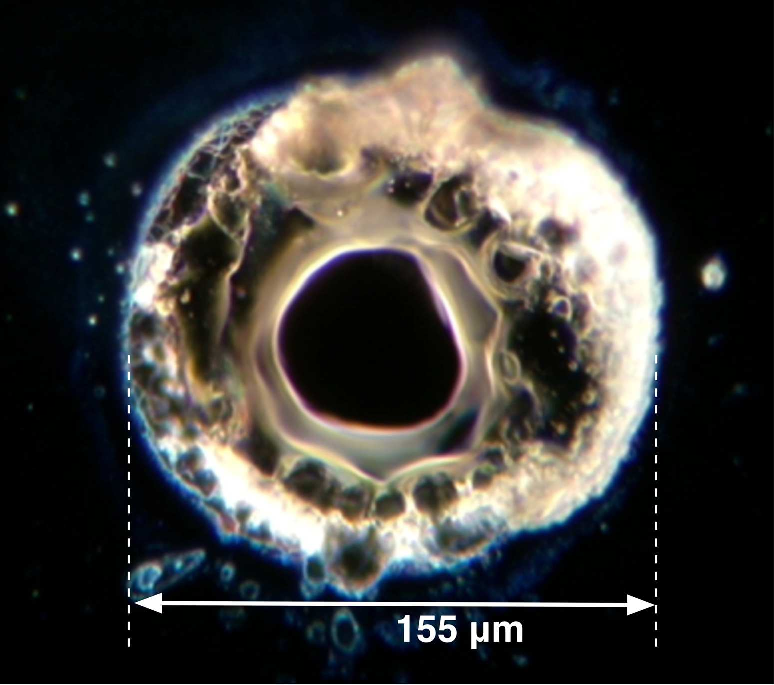
\includegraphics[width=\linewidth]{osafig1}}
% \caption{Dark-field image of a point absorber.}
% \label{fig:false-color}
% \end{figure}

% \subsection{Sample Table}

% Table \ref{tab:shape-functions} shows an example table.

% \begin{table}[htbp]
% \centering
% \caption{\bf Shape Functions for Quadratic Line Elements}
% \begin{tabular}{ccc}
% \hline
% local node & $\{N\}_m$ & $\{\Phi_i\}_m$ $(i=x,y,z)$ \\
% \hline
% $m = 1$ & $L_1(2L_1-1)$ & $\Phi_{i1}$ \\
% $m = 2$ & $L_2(2L_2-1)$ & $\Phi_{i2}$ \\
% $m = 3$ & $L_3=4L_1L_2$ & $\Phi_{i3}$ \\
% \hline
% \end{tabular}
%   \label{tab:shape-functions}
% \end{table}

% \section{Sample Equation}

% Let $X_1, X_2, \ldots, X_n$ be a sequence of independent and identically distributed random variables with $\text{E}[X_i] = \mu$ and $\text{Var}[X_i] = \sigma^2 < \infty$, and let
% \begin{equation}
% S_n = \frac{X_1 + X_2 + \cdots + X_n}{n}
%       = \frac{1}{n}\sum_{i}^{n} X_i
% \label{eq:refname1}
% \end{equation}
% denote their mean. Then as $n$ approaches infinity, the random variables $\sqrt{n}(S_n - \mu)$ converge in distribution to a normal $\mathcal{N}(0, \sigma^2)$.

% \section{Sample Algorithm}

% Algorithms can be included using the commands as shown in algorithm \ref{alg:euclid}.

% \begin{algorithm}
% \caption{Euclid’s algorithm}\label{alg:euclid}
% \begin{algorithmic}[1]
% \Procedure{Euclid}{$a,b$}\Comment{The g.c.d. of a and b}
% \State $r\gets a\bmod b$
% \While{$r\not=0$}\Comment{We have the answer if r is 0}
% \State $a\gets b$
% \State $b\gets r$
% \State $r\gets a\bmod b$
% \EndWhile\label{euclidendwhile}
% \State \textbf{return} $b$\Comment{The gcd is b}
% \EndProcedure
% \end{algorithmic}
% \end{algorithm}

% \subsection{Supplementary materials in Optica Publishing Group journals}
% Optica Publishing Group journals allow authors to include supplementary materials as integral parts of a manuscript. Such materials are subject to peer-review procedures along with the rest of the paper and should be uploaded and described using the Prism manuscript system. Please refer to the \href{https://www.osapublishing.org/submit/style/supplementary_materials.cfm}{Author Guidelines for Supplementary Materials in Optica Publishing Group Journals} for more detailed instructions on labeling supplementary materials and your manuscript. 

% \textbf{Authors may also include Supplemental Documents} (PDF documents with expanded descriptions or methods) with the primary manuscript. At this time, supplemental PDF files are not accepted for JOCN or PRJ. To reference the supplementary document, the statement ``See Supplement 1 for supporting content.'' should appear at the bottom of the manuscript (above the References heading). 

% \begin{figure}[ht!]
% \centering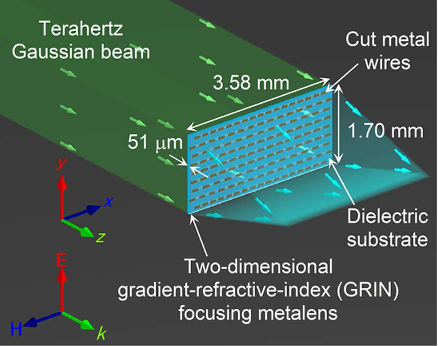
\includegraphics{osafig2}
% \caption{Terahertz focusing metalens.}
% \end{figure}


% \subsection{Sample Dataset Citation}

% 1. M. Partridge, "Spectra evolution during coating," figshare (2014), http://dx.doi.org/10.6084/m9.figshare.1004612.

% \subsection{Sample Code Citation}

% 2. C. Rivers, "Epipy: Python tools for epidemiology," Figshare (2014) [retrieved 13 May 2015], http://dx.doi.org/10.6084/m9.figshare.1005064.

% \section{Backmatter}
% Backmatter sections should be listed in the order Funding/Acknowledgment/Disclosures/Data Availability Statement/Supplemental Document section. An example of backmatter with each of these sections included is shown below.

% \begin{backmatter}
% \bmsection{Funding} Content in the funding section will be generated entirely from details submitted to Prism. Authors may add placeholder text in the manuscript to assess length, but any text added to this section in the manuscript will be replaced during production and will display official funder names along with any grant numbers provided. If additional details about a funder are required, they may be added to the Acknowledgments, even if this duplicates information in the funding section. See the example below in Acknowledgements.

% \bmsection{Acknowledgments} Acknowledgments should be included at the end of the document. The section title should not follow the numbering scheme of the body of the paper. Additional information crediting individuals who contributed to the work being reported, clarifying who received funding from a particular source, or other information that does not fit the criteria for the funding block may also be included; for example, ``K. Flockhart thanks the National Science Foundation for help identifying collaborators for this work.''

% \bmsection{Disclosures} Disclosures should be listed in a separate section at the end of the manuscript. List the Disclosures codes identified on the \href{http://www.osapublishing.org/submit/review/conflicts-interest-policy.cfm}{Conflict of Interest policy page}. If there are no disclosures, then list ``The authors declare no conflicts of interest.''

% \smallskip

% \noindent Here are examples of disclosures:


% \bmsection{Disclosures} ABC: 123 Corporation (I,E,P), DEF: 456 Corporation (R,S). GHI: 789 Corporation (C).

% \bmsection{Disclosures} The authors declare no conflicts of interest.


% \bmsection{Data Availability Statement} A Data Availability Statement (DAS) will be required for all submissions beginning 1 March 2021. The DAS should be an unnumbered separate section titled ``Data Availability'' that
% immediately follows the Disclosures section. See the \href{https://www.osapublishing.org/submit/review/data-availability-policy.cfm}{Data Availability Statement policy page} for more information.

% There are four common (sometimes overlapping) situations that authors should use as guidance. These are provided as minimal models, and authors should feel free to
% include any additional details that may be relevant.

% \begin{enumerate}
% \item When datasets are included as integral supplementary material in the paper, they must be declared (e.g., as "Dataset 1" following our current supplementary materials policy) and cited in the DAS, and should appear in the references.

% \bmsection{Data availability} Data underlying the results presented in this paper are available in Dataset 1, Ref. [3].

% \item When datasets are cited but not submitted as integral supplementary material, they must be cited in the DAS and should appear in the references.

% \bmsection{Data availability} Data underlying the results presented in this paper are available in Ref. [3].

% \item If the data generated or analyzed as part of the research are not publicly available, that should be stated. Authors are encouraged to explain why (e.g.~the data may be restricted for privacy reasons), and how the data might be obtained or accessed in the future.

% \bmsection{Data availability} Data underlying the results presented in this paper are not publicly available at this time but may be obtained from the authors upon reasonable request.

% \item If no data were generated or analyzed in the presented research, that should be stated.

% \bmsection{Data availability} No data were generated or analyzed in the presented research.
% \end{enumerate}

% \bmsection{Supplemental document}
% See Supplement 1 for supporting content. 

% \end{backmatter}

% \section{References}

% Note that \emph{Optics Letters} and \emph{Optica} short articles use an abbreviated reference style. Citations to journal articles should omit the article title and final page number; this abbreviated reference style is produced automatically when the \emph{Optics Letters} journal option is selected in the template, if you are using a .bib file for your references.

% However, full references (to aid the editor and reviewers) must be included as well on a fifth informational page that will not count against page length; again this will be produced automatically if you are using a .bib file.

% \bigskip
% \noindent Add citations manually or use BibTeX. See \cite{Zhang:14,OSA,FORSTER2007,testthesis,manga_rao_single_2007}.


% Bibliography
\bibliography{sample}

% Full bibliography added automatically for Optics Letters submissions; the following line will simply be ignored if submitting to other journals.
% Note that this extra page will not count against page length
\bibliographyfullrefs{sample}

%Manual citation list
%\begin{thebibliography}{1}
%\bibitem{Zhang:14}
%Y.~Zhang, S.~Qiao, L.~Sun, Q.~W. Shi, W.~Huang, %L.~Li, and Z.~Yang,
 % \enquote{Photoinduced active terahertz metamaterials with nanostructured
  %vanadium dioxide film deposited by sol-gel method,} Opt. Express \textbf{22},
  %11070--11078 (2014).
%\end{thebibliography}

% % Please include bios and photos of all authors for aop articles
% \ifthenelse{\equal{\journalref}{aop}}{%
% \section*{Author Biographies}
% \begingroup
% \setlength\intextsep{0pt}
% \begin{minipage}[t][6.3cm][t]{1.0\textwidth} % Adjust height [6.3cm] as required for separation of bio photos.
%   \begin{wrapfigure}{L}{0.25\textwidth}
%     \includegraphics[width=0.25\textwidth]{john_smith.eps}
%   \end{wrapfigure}
%   \noindent
%   {\bfseries John Smith} received his BSc (Mathematics) in 2000 from The University of Maryland. His research interests include lasers and optics.
% \end{minipage}
% \begin{minipage}{1.0\textwidth}
%   \begin{wrapfigure}{L}{0.25\textwidth}
%     \includegraphics[width=0.25\textwidth]{alice_smith.eps}
%   \end{wrapfigure}
%   \noindent
%   {\bfseries Alice Smith} also received her BSc (Mathematics) in 2000 from The University of Maryland. Her research interests also include lasers and optics.
% \end{minipage}
% \endgroup
% }{}

\end{document}
